
\begin{lead}
 一般的に,信号処理を行う前段階として,フィルタ回路が必要となる.このフィルタ回路は電気回路やアナログ電子回路として構成されるが,本章では,基礎的な交流電気回路であるRLC直列回路から理解した上で,高域フィルタや低域フィルタ,帯域フィルタについて,その特性を習得する.

\end{lead}

%\vfill

%\begin{koumoku}
%アナログフィルタ\\
%電気回路\\
%交流電気回路\\
%周波数特性\\
%低域フィルタ\\
%高域フィルタ\\
%帯域フィルタ
%\end{koumoku}

%\clearpage

\chapter{アナログフィルタ}
\label{chapter:a-filter}

\section{交流電気回路:RLC直列電気回路}

ここでは難解な\index{びぶんほうていしき@微分方程式}微分方程式で表される電気回路の電圧電流の関係から,\index{ふくそすう@複素数}複素数を用いた表現に簡略する方法を説明する.

図\ref{fig:rlc0}に示すような\index{RLCちょくれつかいろ@RLC直列回路}RLC直列回路において,電源の両端の電圧$v$と流れる電流$i$との関係\footnotemark は,次式のように表される.
\footnotetext{\index{こうりゅうかいろ@交流回路}交流回路における電圧と電流の関係は,$v_R=Ri$, $\displaystyle v_L=L\frac{di}{dt}$, $\displaystyle v_C=\frac{1}{C} \int idt$と瞬時値による微分方程式で表現される.}
\begin{equation}
v=Ri+L\frac{di}{dt}+\frac{1}{C} \int idt
\label{eqn:denki-rlc}
\end{equation}
このような微分方程式で表されるのだが,\index{ていじょうじょうたい@定常状態}定常状態(スイッチをONにしてから十分時間が経過した状態)であれば,次式のように電圧ならびに電流を複素数
%\footnotemark 
で表す場合,
\begin{equation}
V=V_m \exp{j(\omega t - \theta_v)}
\end{equation}
\begin{equation}
I=I_m \exp{j(\omega t - \theta_i)}
\end{equation}
電流$I$について時間$t$で微分ならびに積分を行うと,
\begin{equation}
\frac{dI}{dt}=j\omega I
\end{equation}
\begin{equation}
\int Idt=\frac{1}{j\omega} I
\end{equation}
となるので,式(\ref{eqn:denki-rlc})は次式のように置き換えることができる.
\begin{equation}
V=\left ( R+j\omega L + \frac{1}{j\omega C} \right ) I
\label{eqn:denki-rlc1}
\end{equation}

%\footnotetext{複素数の扱い\\ 数学の教科書などのように多くの場合 $i=\sqrt{-1}$ と標記するが,電気電子工学や情報工学などの分野では,$i$を電流としての変数として用いるため,混乱を避けるために$j$を用いることとして, $j=\sqrt{-1}$ と標記する慣例がある.}

\begin{figure}[H]
\begin{center}
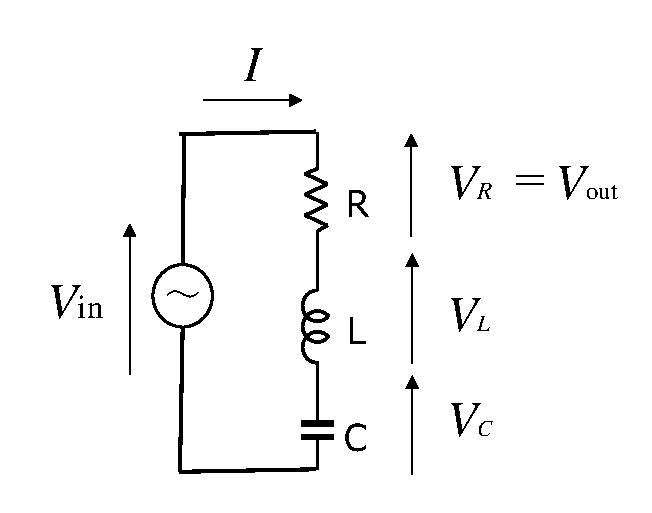
\includegraphics[width=.4\textwidth]{fig/rlc0.eps}
\end{center}
\caption{RLC直列回路}
\label{fig:rlc0}
\end{figure}



\section{高域フィルタ}

図\ref{fig:hpf}に示すようなRC直列回路で,\index{ていこう@抵抗}抵抗Rを出力端とした回路を\index{こういきふぃるた@高域フィルタ}高域フィルタという.高域フィルタとは,低周波の信号を低減して高周波の信号だけを通過させようとするものである.

\begin{figure}[H]
\begin{center}
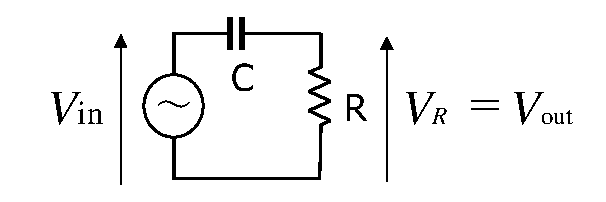
\includegraphics[width=.6\textwidth]{fig/hpf1.eps}
\end{center}
\caption{RC直列回路(高域フィルタ)}
\label{fig:hpf}
\end{figure}

この回路において,入力電圧$V_\textrm{in}$と電流$I$との関係,ならびに出力電圧$V_\textrm{out}$と電流$I$との関係は次式で表される.
\begin{equation}
V_\textrm{in}=\left ( R + \frac{1}{j\omega C} \right ) I
\label{eqn:denki-hpf1}
\end{equation}
\begin{equation}
V_\textrm{out}= R  I
\label{eqn:denki-hpf2}
\end{equation}

このRC直列回路における入力と出力との関係を\index{でんたつかんすう@伝達関数}伝達関数$T(\omega)$で表すと,
\begin{equation}
T(\omega)  = \frac{V_\textrm{out}}{V_\textrm{in}} 
= \frac{R}{\displaystyle R + \frac{1}{j\omega C}}
= \frac{j\omega CR}{1 + j\omega CR} \label{eqn:hanbunsu_1}
\end{equation}
である\footnotemark .実際には,まず\index{かくしゅうはすう@角周波数}角周波数$\omega$の変化に対する$T(\omega)$の大きさ$|T(\omega)|$の変化がわかるとよいので,
\begin{equation}
|T(\omega)| = \left | \frac{j\omega CR}{1 + j\omega CR} \right | 
= \displaystyle \sqrt{\frac{\omega^2 C^2 R^2}{1 + \omega^2 C^2 R^2}}
\end{equation}
と書き換える.ここで,角周波数が0のときと$\infty$のときの$T(\omega)$を計算すると,
\footnotetext{式(\ref{eqn:hanbunsu_1})のような複雑な分数式(繁分数式\index{はんぶんすうしき@繁分数式})は,$T(\omega)  =  \displaystyle \frac{R}{\displaystyle R + \frac{1}{j\omega C}}  =  \displaystyle \frac{R \times j\omega C}{\displaystyle \left (R + \frac{1}{j\omega C} \right ) \times j\omega C}  = \displaystyle \frac{j\omega CR}{1 + j\omega CR} $として簡単化を行う.}
\begin{equation}
|T(0)| = \lim_{\omega \rightarrow 0} \displaystyle \sqrt{\frac{\omega^2 C^2 R^2}{1 + \omega^2 C^2 R^2}}  = 0
\end{equation}
\begin{equation}
|T(\infty)| = \lim_{\omega \rightarrow \infty}\displaystyle \sqrt{\frac{\omega^2 C^2 R^2}{1 + \omega^2 C^2 R^2}} 
 = \lim_{\omega \rightarrow \infty}\displaystyle \sqrt{\frac{2\omega C^2 R^2}{ 2\omega C^2 R^2}} 
 = \lim_{\omega \rightarrow \infty}\displaystyle \sqrt{\frac{2 C^2 R^2}{ 2 C^2 R^2}}  = 1
\end{equation}
となる.このことから,周波数が低い場合($\omega$が小さく0に近づく場合)は$|T(\omega)|$は0に近づくので,低周波領域は遮断されているということができる.逆に周波数が低い場合($\omega$が大きく$\infty$に近づく場合)は$|T(\omega)|$は1に近づくので,高周波領域は通過しているということができる\footnotemark .このため,高域を通過させるフィルタということで,高域フィルタと呼ぶのである.

\footnotetext{ロピタルの定理は,分数式の極限を求める際に,分母と分子がともに0になるか,分母と分子がともに無限大になる場合の極限値を求める方法であり,
$\lim_{x \rightarrow c}\frac{f(x)}{g(x)}  =  \lim_{x \rightarrow c}\frac{f'(x)}{g'(x)}  =  L$
なる方法で有限の極限値を求めることができる.
}

このフィルタにおいて$|T(\omega)|$が$1/\sqrt{2}$となる周波数$\omega_c$をカットオフ周波数(遮断周波数)と呼ぶ.この\index{こういきふぃるた@高域フィルタ}高域フィルタの場合には\index{かっとおふしゅうはすう@カットオフ周波数}カットオフ周波数$\omega_c$は,
\begin{equation}
|T(\omega_c)|  =  \displaystyle \sqrt{\frac{{\omega_c}^2 C^2 R^2}{1 + {\omega_c}^2 C^2 R^2}}  =  \sqrt{\frac{1}{2}}
\end{equation}
における$\omega_c$を求めればよいので,両辺の根号の内部を見ると,
\begin{equation}
\frac{{\omega_c}^2 C^2 R^2}{1 + {\omega_c}^2 C^2 R^2}  =  \frac{1}{2}
\end{equation}
となるので,この式を整理すると,
\begin{equation}
\omega_c^2 C^2 R^2 = 1
\end{equation}
となることから
\begin{equation}
\omega_c = \frac{1}{CR}
\end{equation}
となる.ここで求まった$\omega_c$より高い周波数は通過して$\omega_c$より低い周波数を遮断する高域フィルタであるということができる.

\section{\index{ていいきふぃるた@低域フィルタ}低域フィルタ}

図\ref{fig:lpf2}に示すような\index{RCちょくれつかいろ@RC直列回路}RC直列回路で,\index{こんでんさ@コンデンサ}コンデンサCを出力端とした回路を低域フィルタという.低域フィルタとは,高周波の信号を低減して低周波の信号だけを通過させようとするものである.
\begin{figure}[H]
\begin{center}
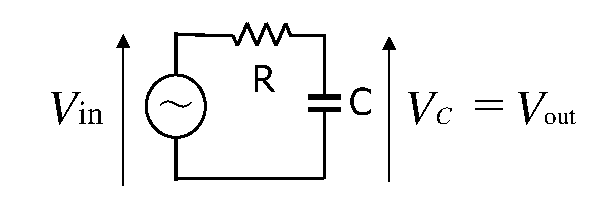
\includegraphics[width=.6\textwidth]{fig/lpf1.eps}
\end{center}
\caption{RC直列回路(低域フィルタ)}
\label{fig:lpf2}
\end{figure}

この回路において,入力電圧$V_\textrm{in}$と電流$I$との関係,ならびに出力電圧$V_\textrm{out}$と電流$I$との関係は次式で表される.
\begin{equation}
V_\textrm{in}=\left ( R + \frac{1}{j\omega C} \right ) I
\label{eqn:denki-lpf1}
\end{equation}
\begin{equation}
V_\textrm{out}= \frac{1}{j\omega C}  I
\label{eqn:denki-lpf2}
\end{equation}

このRC直列回路における入力と出力との関係を伝達関数$T(\omega)$で表すと,
\begin{equation}
T(\omega)  =  \frac{V_\textrm{out}}{V_\textrm{in}} 
 = \frac{\displaystyle \frac{1}{j\omega C}}{\displaystyle R + \frac{1}{j\omega C}} 
 = \frac{1}{1 + j\omega CR}
\end{equation}
である.実際には,まず角周波数$\omega$の変化に対する$T(\omega)$の大きさ$|T(\omega)|$の変化がわかるとよいので,
\begin{equation}
|T(\omega)| = \left | \frac{1}{1 + j\omega CR} \right | 
 =  \displaystyle \sqrt{\frac{1}{1 + \omega^2 C^2 R^2}}
\end{equation}
と書き換える.ここで,角周波数が0のときと$\infty$のときの$T(\omega)$を計算すると,
\begin{equation}
|T(0)| = \lim_{\omega \rightarrow 0} \displaystyle \sqrt{\frac{1}{1 + \omega^2 C^2 R^2}}  =  1
\end{equation}
\begin{equation}
|T(\infty)|  =  \lim_{\omega \rightarrow \infty}\displaystyle \sqrt{\frac{1}{1 + \omega^2 C^2 R^2}}  =  0
\end{equation}
となる.このことから,周波数が低い場合($\omega$が小さく0に近づく場合)は$|T(\omega)|$は0に近づくので,低周波領域は遮断されているということができる.逆に周波数が低い場合($\omega$が大きく$\infty$に近づく場合)は$|T(\omega)|$は1に近づくので,高周波領域は通過しているということができる.このため,高域を通過させるフィルタということで,高域フィルタと呼ぶのである.

このフィルタにおいて$|T(\omega)|$が$1/\sqrt{2}$となる周波数$\omega_c$をカットオフ周波数(遮断周波数)と呼ぶ.この高域フィルタの場合にはカットオフ周波数$\omega_c$は,
\begin{equation}
|T(\omega_c)|  = \displaystyle \sqrt{\frac{{\omega_c}^2 C^2 R^2}{1 + {\omega_c}^2 C^2 R^2}}  =  \sqrt{\frac{1}{2}}
\end{equation}
における$\omega_c$を求めればよいので,両辺の根号の内部を見ると,
\begin{equation}
\frac{{\omega_c}^2 C^2 R^2}{1 + {\omega_c}^2 C^2 R^2}  =  \frac{1}{2}
\end{equation}
となるので,この式を整理すると,
\begin{equation}
\omega_c^2 C^2 R^2 = 1
\end{equation}
となることから
\begin{equation}
\omega_c = \frac{1}{CR}
\end{equation}
となる.ここで求まった$\omega_c$より低い周波数は通過して,$\omega_c$より高い周波数を遮断する低域フィルタであるということができる.

\section{帯域フィルタ}

ここでは図\ref{fig:rlc01}に示すRLC直列回路において,Rを出力端とした場合を考え,帯域フィルタとなることを説明する.

\begin{figure}[H]
\begin{center}
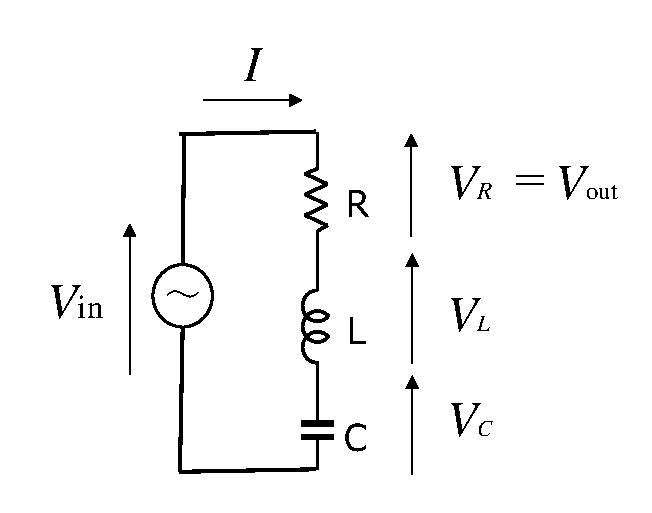
\includegraphics[width=.4\textwidth]{fig/rlc0.eps}
\end{center}
\caption{帯域フィルタ}
\label{fig:rlc01}
\end{figure}

図\ref{fig:rlc01}に示すようなRLC直列回路において入力電圧$V_\textrm{in}$と出力電圧$V_\textrm{out}$との関係は次式のように表される.
\begin{equation}
V_\textrm{in}=\left ( R+j\omega L + \frac{1}{j\omega C} \right ) I
\label{eqn:denki-bpf1}
\end{equation}
\begin{equation}
V_\textrm{out} = R I
\label{eqn:denki-bpf2}
\end{equation}

この2つの式より,伝達関数$T(\omega)$は,
\begin{equation}
T(\omega)  =  \frac{V_\textrm{out}}{V_\textrm{in}} 
 = \frac{\displaystyle R}{\displaystyle R + j \omega L + \frac{1}{j\omega C}}
  = \frac{j\omega CR}{1-\omega^2LC + j\omega CR}
\end{equation}
となる.この場合であるが,伝達関数の大きさ$|T(\omega)|$が最大となる$\omega$を求めると,
\begin{equation}
\frac{d|T(\omega)|}{d\omega}=0
\end{equation}
を満足する$\omega$であることから,
\begin{equation}
\omega_0 = \frac{1}{\sqrt{LC}}
\end{equation}
である.この$\omega_0$を中心とした周波数の信号を通過させ,それよりも非常に高い周波数や非常に低い周波数の信号を遮断することができるため,このフィルタを帯域フィルタと呼ぶのである.

この角周波数$\omega$と$|T(\omega)|$との関係を図\ref{fig:bpf-graph}に示す.$\omega_0$で$|T(\omega)|$が最大となることがわかる.なお,縦軸も横軸も対数表示をすると直線状の変化となることがわかる.

\begin{figure}[H]
\begin{center}
\begin{minipage}{.36\textwidth}
\begin{center}
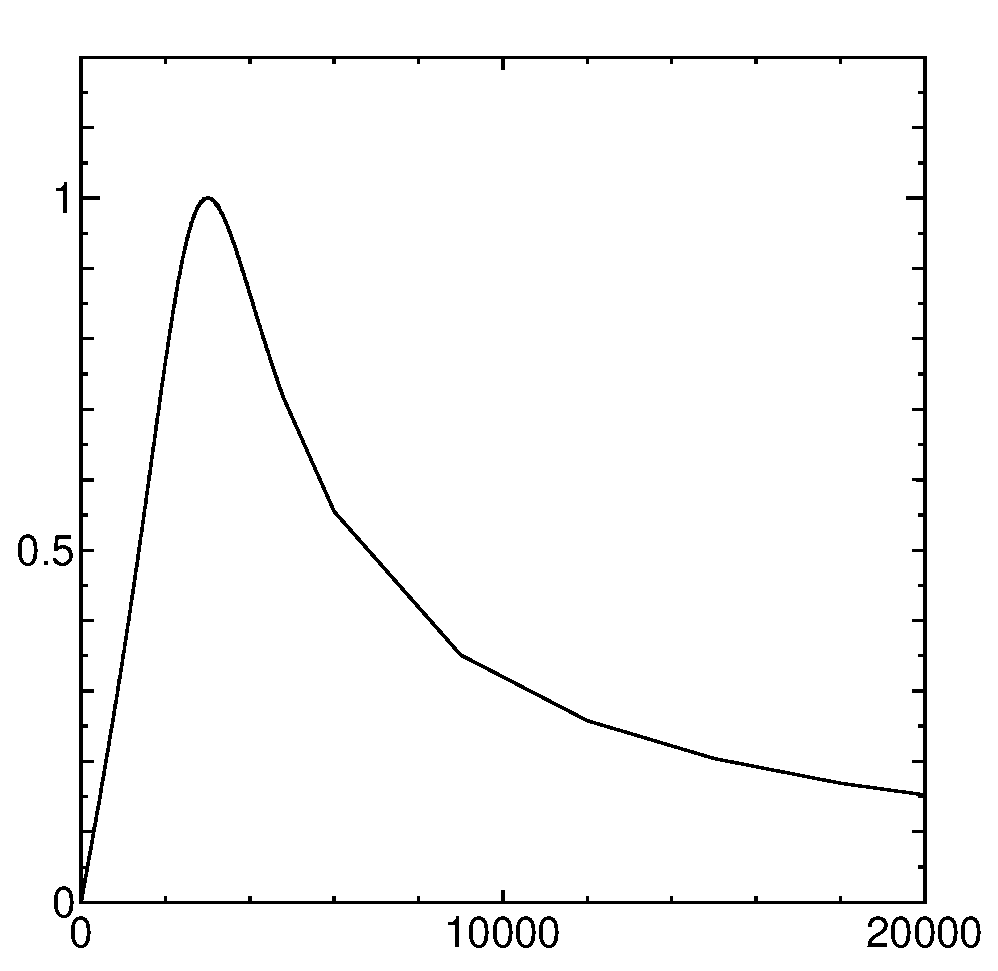
\includegraphics[width=.98\textwidth]{fig/filter-bpf-n2.eps}

(a) 横軸,縦軸ともにlinear表示
\end{center}
\end{minipage}
\begin{minipage}{.36\textwidth}
\begin{center}
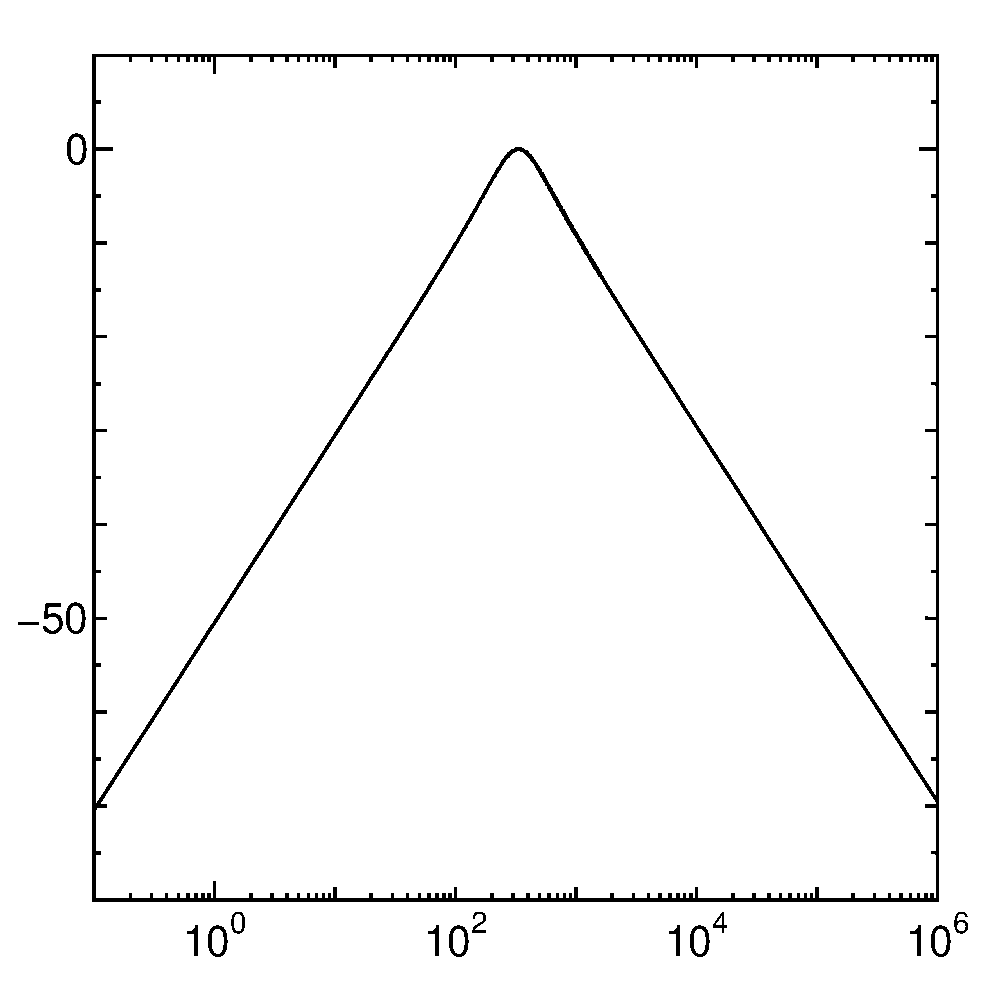
\includegraphics[width=.98\textwidth]{fig/filter-bpf-log3.eps}

(b) 横軸,縦軸ともにlog表示
\end{center}
\end{minipage}
\end{center}\vskip.5\baselineskip
\caption{\index{ばんどぱすふぃるた@バンドパスフィルタ}バンドパスフィルタの周波数特性}
\label{fig:bpf-graph}
\end{figure}


\section*{演習問題}

\subsection*{問題\ref{chapter:a-filter}.1}

図\ref{fig:hpf}に示す高域フィルタおいて,カットオフ周波数$\omega_c$におけるゲインはいくらか.単位は[dB]で示すものとし,ゲインの最大値は0dBであるものとする.

(ヒント:単位を[dB]で表すときは,ゲイン$G$は$G=20\log_{10} (V_\textrm{out}/V_\textrm{in})$として計算する)

\subsection*{問題\ref{chapter:a-filter}.2}

図\ref{fig:hpf}に示す低域フィルタおいて,カットオフ周波数$\omega_c$を1kHzに選びたい.抵抗$R=10\textrm{k}\Omega$とした場合,コンデンサ$C$の容量はいくらか.

\subsection*{問題\ref{chapter:a-filter}.3}

図\ref{fig:rlc01}に示す帯域フィルタおいて,共振周波数$\omega_c$を1MHzに選びたい.インダクタンス$L=1\textrm{mH}$とした場合,コンデンサ$C$の容量はいくらか.

\subsection*{問題\ref{chapter:a-filter}.4}

図\ref{fig:rlc_p}に示すRLC並列回路における入力電圧$V_\textrm{in}$と電流$I$との関係を示せ.\\(ヒント:\index{きるひほっふのほうそく@キルヒホッフの法則}キルヒホッフの法則)

\begin{figure}[H]
\begin{center}
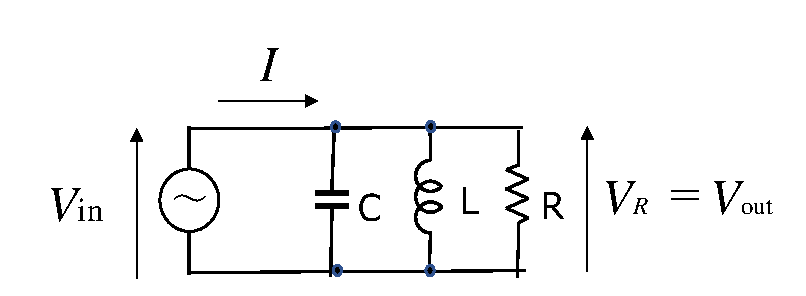
\includegraphics[width=.6\textwidth]{fig/rlc_p.eps}
\end{center}
\caption{\index{RLCへいれつかいろ@RLC並列回路}RLC並列回路}
\label{fig:rlc_p}
\end{figure}


